%%%%%%%%%%%%%%%%%%%%%%%%%%%%%%%%%%%%%%%%%%

\chapter{Tests of the second switcher and switcher wye on the West Beamline}\label{chap:fall2021}

%%%%%%%%%%%%%%%%%%%%%%%%%%%%%%%%%%%%%%%%%%

In 2021, the ongoing construction of the\acrshort{msr} (Sec.~\ref{sec:MSR}) relegated the commissioning of nEDM components to the West beamline (Fig.~\ref{fig:AreaB_schematic}). A second rotary switcher and a new ``switcher wye'' guide segment for connecting both switchers to the beamline (Fig.~\ref{subfig:switcher_mockup}) were tested. This chapter present

%%%%%%%%%%%%%%%%%%%%%%%%%%%%%%%%%%%%%%%%%%%%%%

\section{Description of experimental setup (2021)}

%%%%%%%%%%%%%%%%%%%%%%%%%%%%%%%%%%%%%%%%%%%%%%

UCN tau roundhouse. A buffer volume called the ``roundhouse'' was introduced in 2018 that  smooths over any temporal fluctuations in the UCN production rate while loading

New Y. NiP coated Vertical separation (center to center of beamline) $\qty{18.85}{in}\approx\qty{0.48}{m}$. Corresponds to a $\sim \qty{25}{neV}$ potential step for upper switcher and a boost to the lower switcher. 

Coils and solenoids (depicted in Fig.~\ref{subfig:west_beamline_switchers}) again keep everything under $\sim \qty{1}{mT}$ field. Describe roundhouse field coil

A second switcher had been constructed for this measurement cycle, was placed on the lower side of the switcher stand. Off this side was the single channel spin analyzer used in Chap.~\ref{chap:north_beamline_paper} and \ref{chap:lanl_ramsey_demonstration}. On the higher switcher was a simultaneous spin analyzer (SSA). Be clear about which switcher is new, which switcher is higher, which switcher has what spin analyzer (maybe use a table?)

\begin{figure}
    \centering
    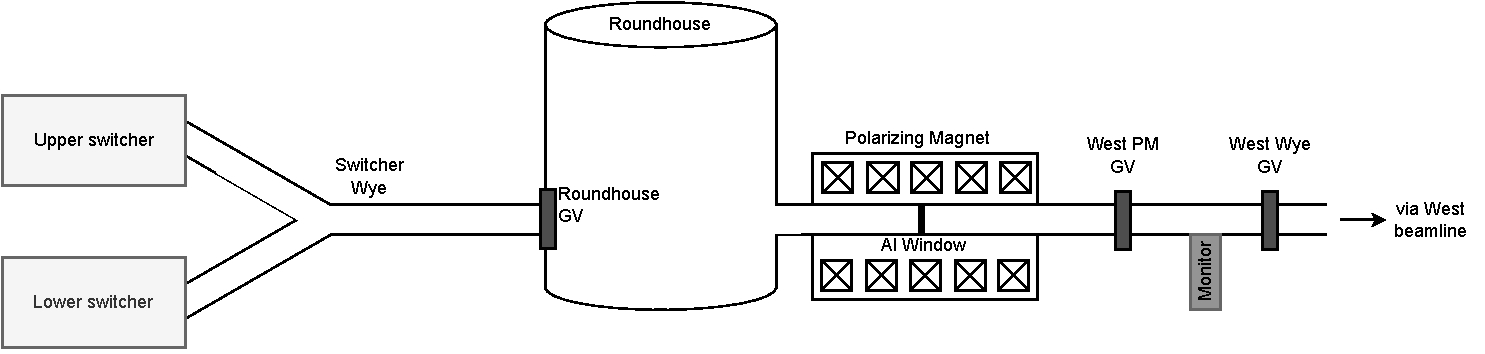
\includegraphics[width=\textwidth]{figures/westbeamline_2021.pdf}
    \caption[West beamline configuration for measurements in 2021.]
    {West beamline configuration for measurements in 2021. A single channel spin analyzer was located on the lower switcher, and simultaneous spin analyzer was located on the upper switcher. Beam height detectors were rearranged for different measurements as per Sec.~\ref{sec:2021_ucn_transport_switchers}.}\label{fig:west_beamline_2021}
\end{figure}

\begin{figure}
\centering
%subfigure width gets "multiplied" by includegraphics width
\begin{subfigure}{.5\textwidth}
  \centering
  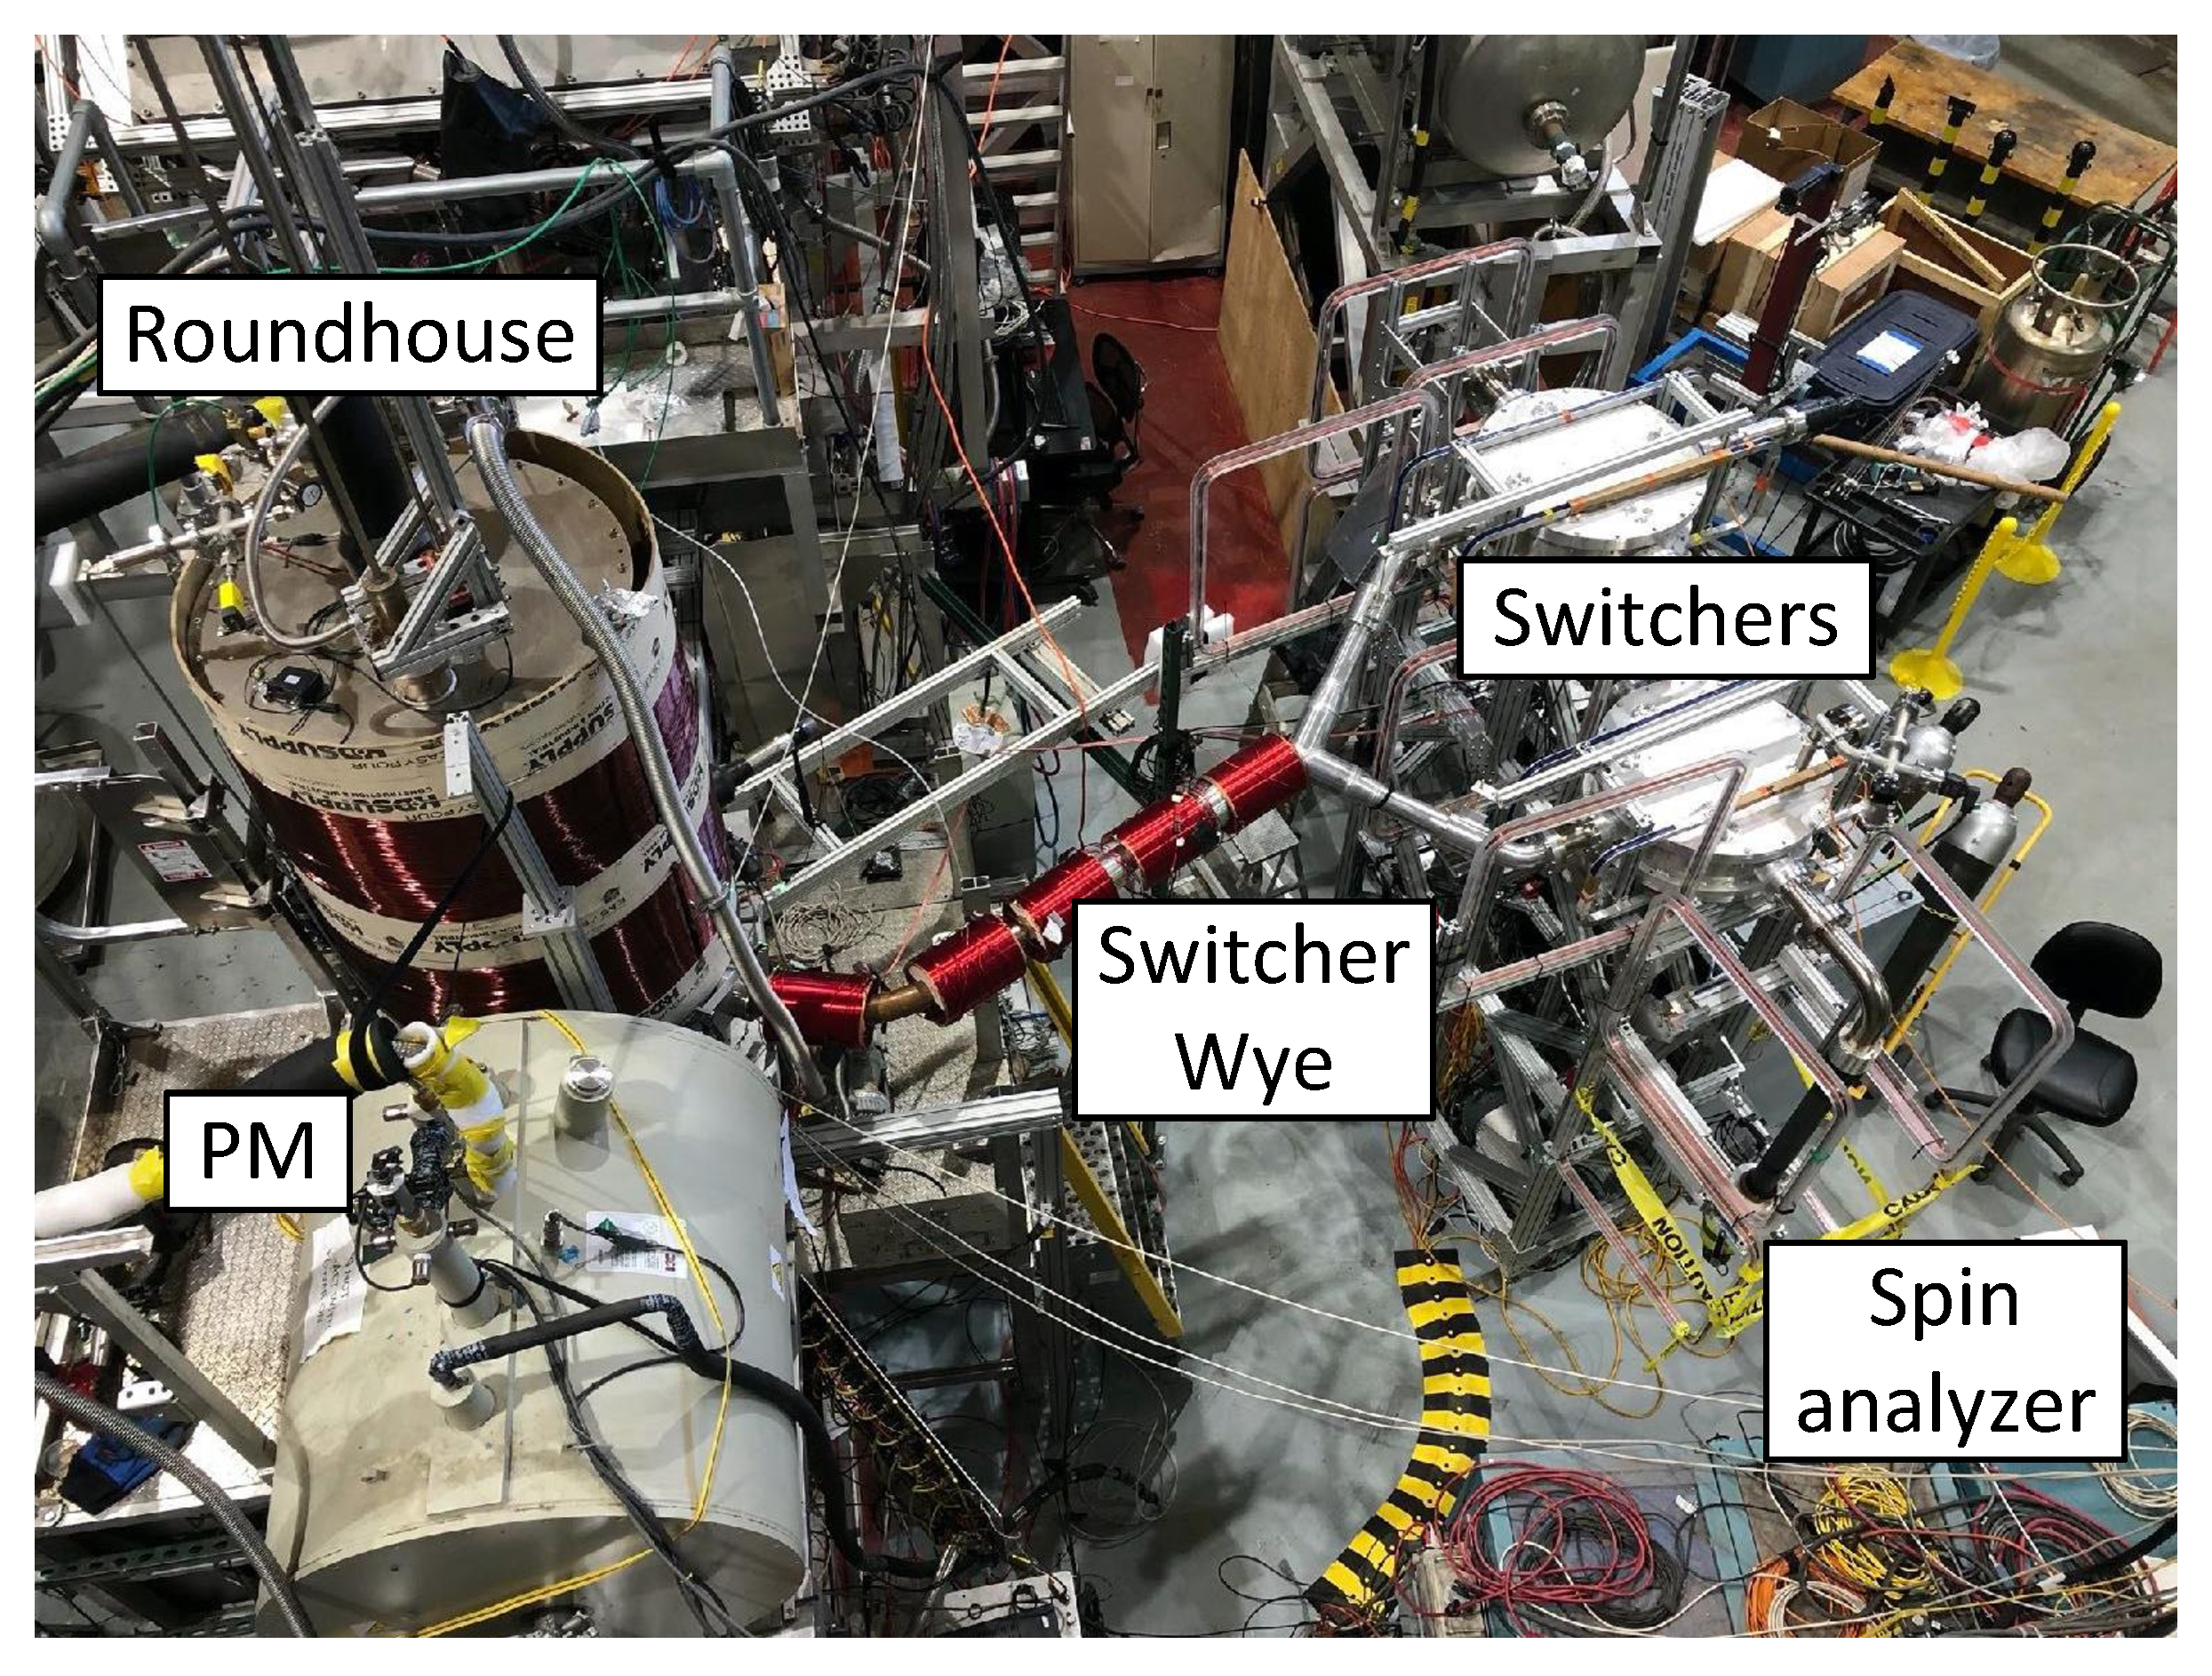
\includegraphics[width=\textwidth]{figures/2021_west_beamline_image.pdf}
  \vspace{5pt}
  \caption{}\label{subfig:west_beamline_switchers}
\end{subfigure}%DO NOT REMOVE THIS '%'
\begin{subfigure}{.5\textwidth}
  \centering
  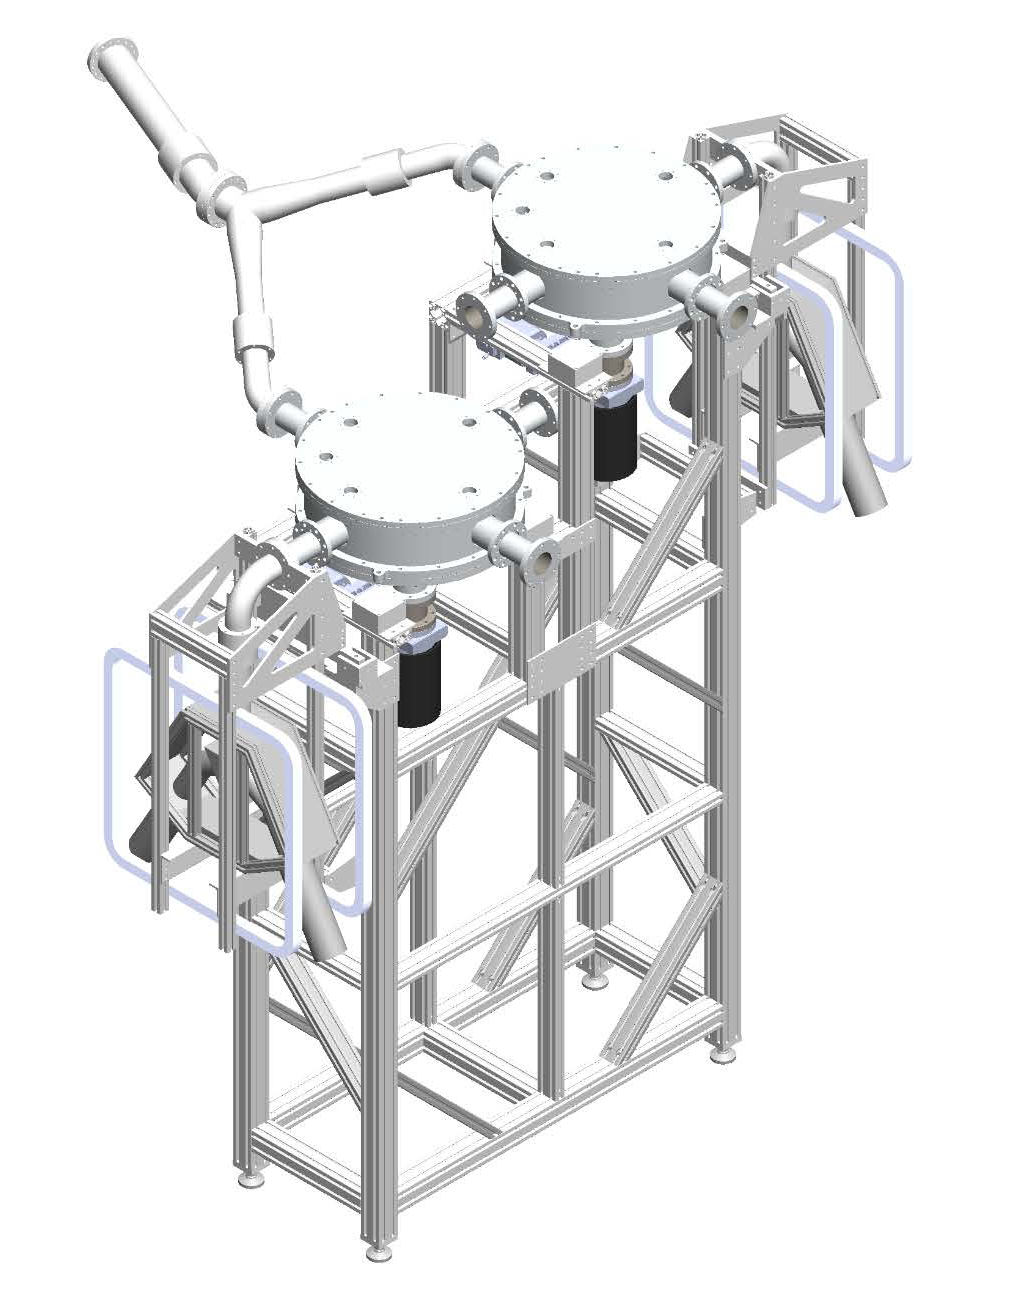
\includegraphics[height=3in]{figures/switcher_mockup.png}
  \caption{}\label{subfig:switcher_mockup}
\end{subfigure}
\caption
{\textbf{(\subref{subfig:west_beamline_switchers})} Image of the experimental setup on the West beamline. \textbf{(\subref{subfig:switcher_mockup})} Rendering of the switcher wye, switcher stand, and switcher, depicted here with simultaneous spin analyzers attached.}
\label{fig:west_beamline_switchers}
\end{figure}



%%%%%%%%%%%%%%%%%%%%%%%%%%%%%%%%%%%%%%%%%%%%%%

\section{UCN transport measurements}\label{sec:2021_ucn_transport_switchers}

%%%%%%%%%%%%%%%%%%%%%%%%%%%%%%%%%%%%%%%%%%%%%%

\begin{figure}
\centering
%subfigure width gets "multiplied" by includegraphics width
\begin{subfigure}{.5\textwidth}
  \centering
  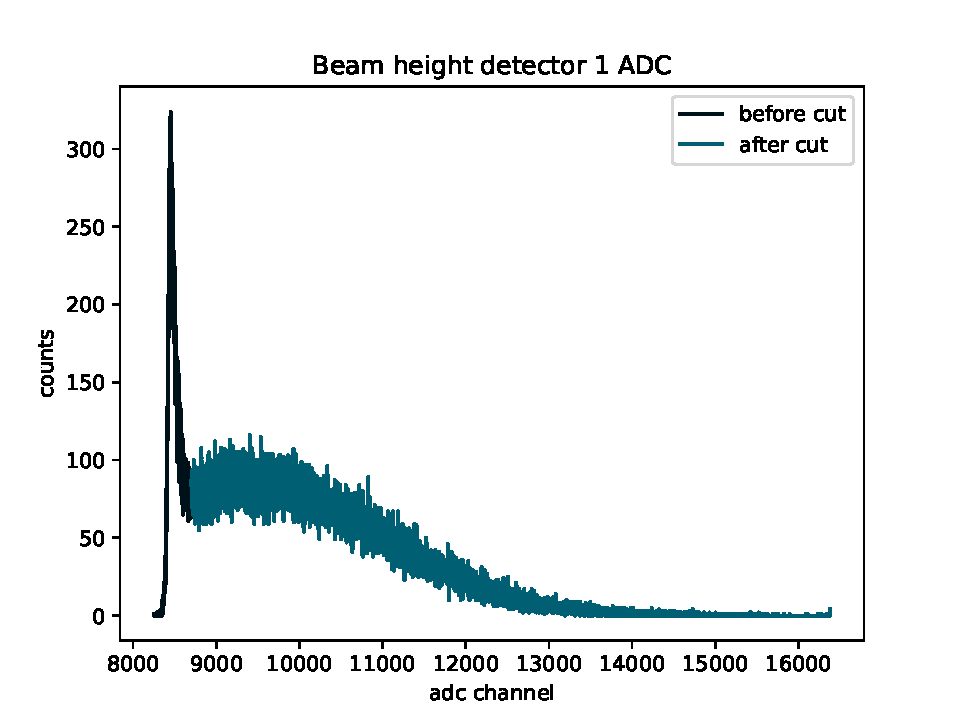
\includegraphics[width=\textwidth]{figures/2021_beam_det_1_adc.pdf}
  \caption{}\label{subfig:beam_det_1_adc}
\end{subfigure}%DO NOT REMOVE THIS '%'
\begin{subfigure}{.5\textwidth}
  \centering
  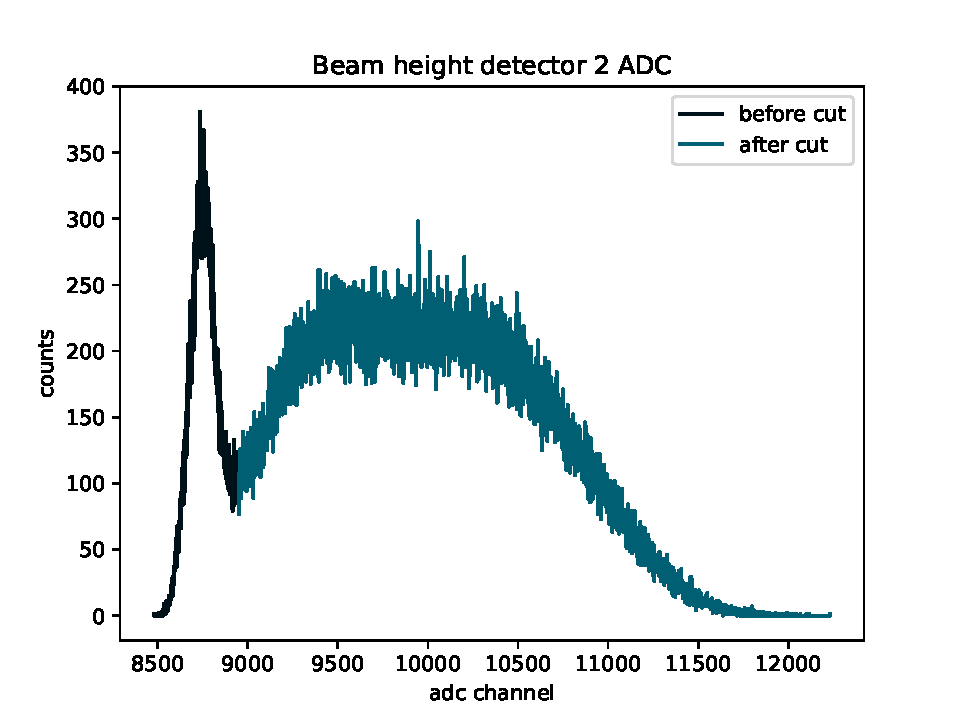
\includegraphics[width=\textwidth]{figures/2021_beam_det_2_adc.pdf}
  \caption{}\label{subfig:beam_det_2_adc}
\end{subfigure}
\begin{subfigure}{.5\textwidth}
  \centering
  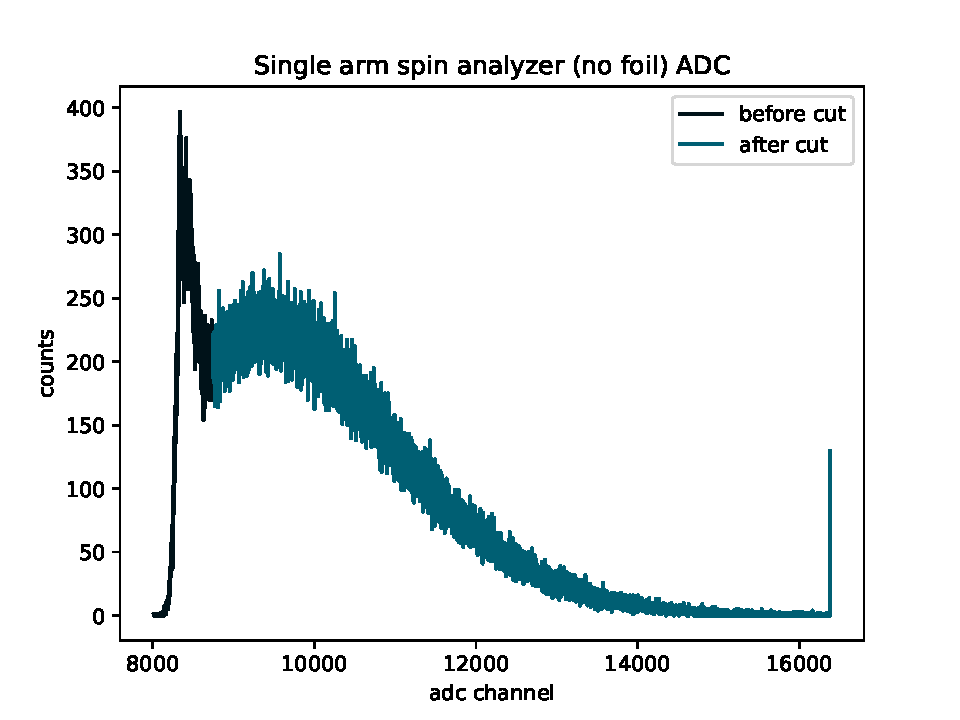
\includegraphics[width=\textwidth]{figures/2021_single_arm_no_foil_adc.pdf}
  \caption{}\label{subfig:single_arm_no_foil_adc}
\end{subfigure}
\caption
[Peak height spectra from \BZnS scintillator and PMT detectors (additional data acqusition details in Chap.~\ref{chap:daq}).  Data cuts selected as per Ref.~\cite{jeph_multilayer_2015}.]
{Peak height spectra from \BZnS scintillator and PMT detectors (additional data acqusition details in Chap.~\ref{chap:daq}). Data cuts selected as per Ref.~\cite{jeph_multilayer_2015}. \textbf{(\subref{subfig:beam_det_1_adc})}--\textbf{(\subref{subfig:beam_det_2_adc})} Beam height detectors. \textbf{(\subref{subfig:single_arm_no_foil_adc})} Single arm spin analyzer with polarizing foil removed. The largest bin in the histogram $x$-axis ($2^{14}-1$) includes counts of pulse heights greater than the range of the histogram}
\label{fig:2021_detector_adc}
\end{figure}

Show ADC cuts for each detector. Spectrum did not change when detectors were moved. As is typical for the UCN spectrum from BZs we make cuts at the noise peak~\cite{jeph_multilayer_2015}

2x 3 inch BnZS scintillator (Sec.~\ref{sec:ucn_detectors})  + PMTs at beam height. 

\begin{small}
\begin{verbatim}
Both PMTs beam height on switcher 1 (higher switcher)
======================================================
SINGLE CHANNEL DET FOIL OUT
detector rate: 1443.88
wgv rate: 632.46
normalized to wgv 650 [Hz]: 1483.9230939506056

BEAM HEIGHT DET: WEST TEST PORT
detector rate: 1435.18
wgv rate: 641.26
normalized to wgv 650 [Hz]: 1454.7406668122135

BEAM HEIGHT DET: STRAIGHT THROUGH
detector rate: 1498.215
wgv rate: 635.39
normalized to wgv 650 [Hz]: 1532.6645839563103

Beam height PMTs on both switchers
======================================================
SINGLE CHANNEL DET FOIL OUT
detector rate: 1465.2666666666667
wgv rate: 656.6
normalized to wgv 650 [Hz]: 1450.5381256980404

BEAM HEIGHT DET: SWITCHER 2 (LOWER)
detector rate: 2244.225
wgv rate: 650.0416666666666
normalized to wgv 650 [Hz]: 2244.0811486443176

BEAM HEIGHT DET: SWITCHER 1 (HIGHER)
detector rate: 1512.1142857142856
wgv rate: 649.5142857142857
normalized to wgv 650 [Hz]: 1513.2450622443143

Switcher 2 transmission difference: 1.5425987599300384
\end{verbatim}
\end{small}

While a factor of 1.5 is unintuitive, PENTrack simulations indicate this is achievable in the current geometry

%%%%%%%%%%%%%%%%%%%%%%%%%%%%%%%%%%%%%%%%%%%%%%

\section{Spin asymmetry measurement with single arm spin analyzer}\label{sec:single_arm_flow_through_west_2021}

%%%%%%%%%%%%%%%%%%%%%%%%%%%%%%%%%%%%%%%%%%%%%%

Single arm spin analyzer on the lower detector. Upper switcher had the SSA. 

Low contrast observed in a flow through mode measurement from the source to previously-proven the single arm detector. (very close to 0 is bad. Asymmetry = $\pm 1$ if everything is polarized) Need to rule out switcher depolarization! It was discovered that the roundhouse was depolarizing due to small patches of exposed stainless steel on some gate valves. 

In discussion with UCNtau collaborators this asymmetry was roughly consistent with measurements they did.

\begin{tiny}
\begin{verbatim}
    21:34 Production run #21184: 20s hold, AFP 0ff, RH coil  On; dagger unload: 2,175; RH dump: 267,712, Yield: 0.0081
*****Spin contrast (on/off) = 2.06 : 1 = 1: 0.48; depolarization = 1/3 = 33%, or the trapping efficiency is 67%. ********** 
21:45 Production run #21185: 20s hold, AFP 0ff, RH coil  On; dagger unload: 2,041; RH dump: 263,671, Yield: 0.0077 
21:57 Production run #21186: 20s hold, AFP 0ff, RH coil Off; dagger unload: 2,447; RH dump: 274,794, Yield: 0.0089
22:09 Production run #21187: 20s hold, AFP  On, RH coil Off; dagger unload: 4,093; RH dump: 258,829, Yield: 0.0158
*****Spin contrast (on/off), RH coill off = 1.77 : 1 = 1: 0.56; depolarization = 36%, or the trapping efficiency is 64%. **********
\end{verbatim}
\end{tiny}

 By comparison, a direct flow through mode measurement from the \ucn source to the spin analyzer (Fig.~\ref{fig:spin_flipper_efficiency}) gives $A(0)\approx 0.8$.

 Also note that the peak has shifted to 22 kHz


%%%%%%%%%%%%%%%%%%%%%%%%%%%%%%%%%%%%%%%%%%%%%%

\section{Roundhouse fill and unload time }

%%%%%%%%%%%%%%%%%%%%%%%%%%%%%%%%%%%%%%%%%%%%%%


\begin{figure}

\end{figure}

\begin{figure}
\centering
\begin{minipage}{.47\textwidth}
    \centering
    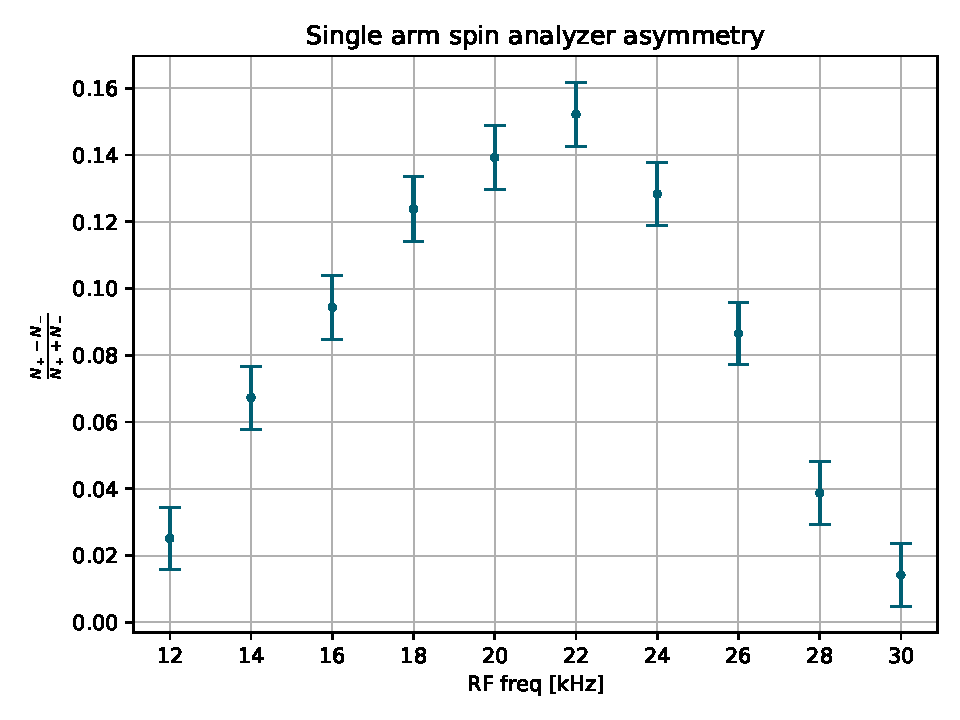
\includegraphics[width=\textwidth]{figures/single_arm_asymmetry_2021.pdf}
    \caption
    {Spin asymmetry measurement from the single arm analyzer, with UCN in a flow through mode from the source through the roundhouse to the detector (Sec.~\ref{sec:single_arm_flow_through_west_2021}).}
    \label{fig:2021_west_single_arm_asymmetry}
\end{minipage}%
\hspace{7pt}
\begin{minipage}{.47\textwidth}
    \centering
    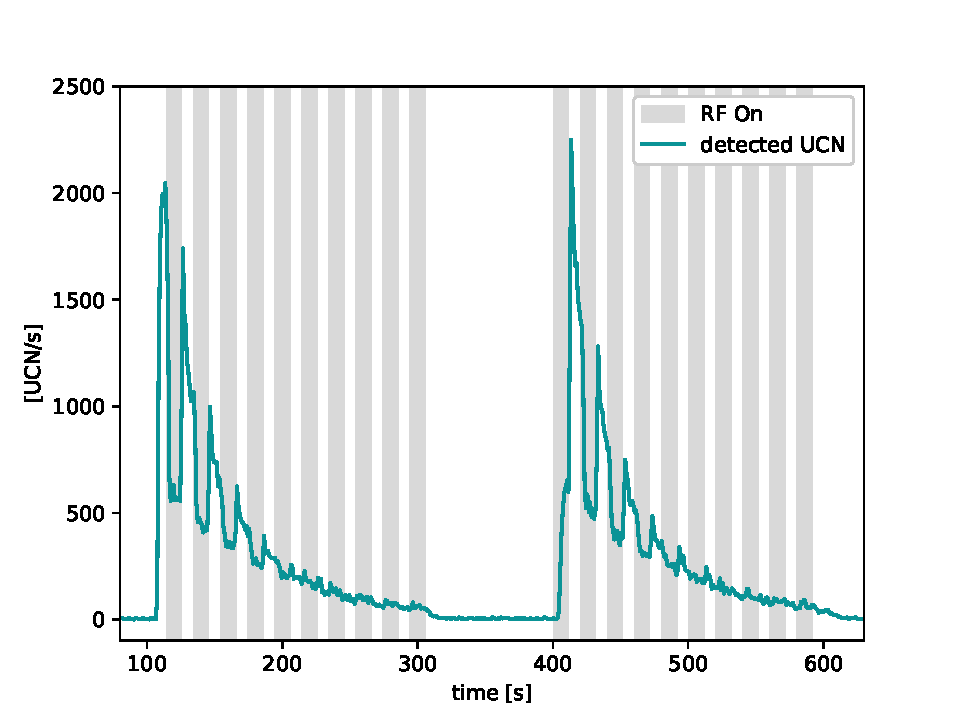
\includegraphics[width=\textwidth]{figures/2021_roundhouse_rf_toggle.pdf}
    \caption
    {Neutron count rate from a fill-and-dump run doublet from the roundhouse on the West beamline with the RF spin flipper toggling.}
    \label{fig:roundhouse_rf_toggle_doublet}
\end{minipage}
\end{figure}

 To extract performance on the behavior of the spin analyzers, a method similar to the T1 measurement in Chap.~\ref{chap:lanl_ramsey_demonstration}. Describe fill and dump with roundhouse. No preload period against WGV. Roundhouse filling time swept. RH Gate valve was then opened. During the 200 s it took to drain the large volume of the RH, spin flipper was toggling every 10 seconds

Observed that as filling time increased, asymmetry decreased. 

Figure~\ref{fig:2021_roundhouse_asymmetry_2} replots the information in Fig.~\ref{fig:2021_roundhouse_asymmetry_1} in a different way. As unload time increases that tells you how many integration periods over the run you sum (20s means you've summed the first two, 30 means you've summed the first 3, etc.). As you allow the unload to continue asymmetry decreases, because UCN get multiple trips back to the roundhouse.

 \begin{figure}
    \centering
    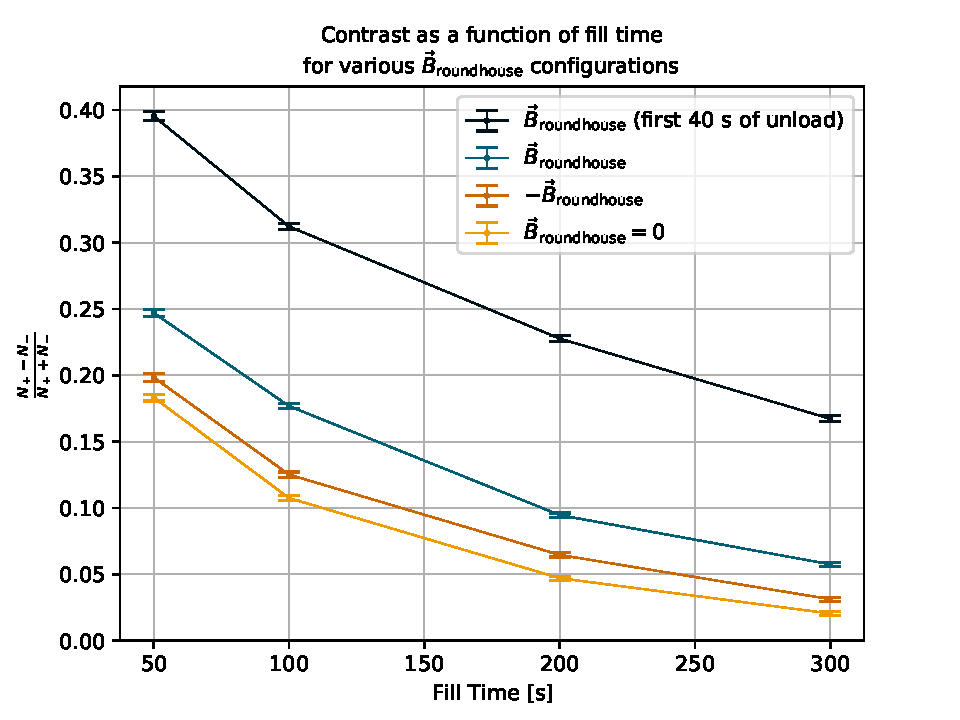
\includegraphics[width=0.6\textwidth]{figures/2021_roundhouse_asymmetry_1.pdf}
    \caption
    [Spin asymmetry from a fill-and-dump sequence of the roundhouse, where fill time was swept. The measurement was repeated for various orientations of the roundhouse magnetic holding field.]
    {Spin asymmetry from a fill-and-dump sequence of the roundhouse, where fill time was swept. The measurement was repeated for various configurations of the roundhouse magnetic holding field: nominal ($\vv{B}_\text{roundhouse}$), inverted along $z$ ($-\vv{B}_\text{roundhouse}$), and off ($\vv{B}_\text{roundhouse}=0$). The \legendbox{black} points labeled ``first 40 s of unload'' use the same data as the nominal configuration \legendbox{dark-blue-color}, but consider only the first 4 integration periods of the run doublet.}
    \label{fig:2021_roundhouse_asymmetry_1}
% \end{figure}
    \vspace{\baselineskip}
% \begin{figure}
    \centering
    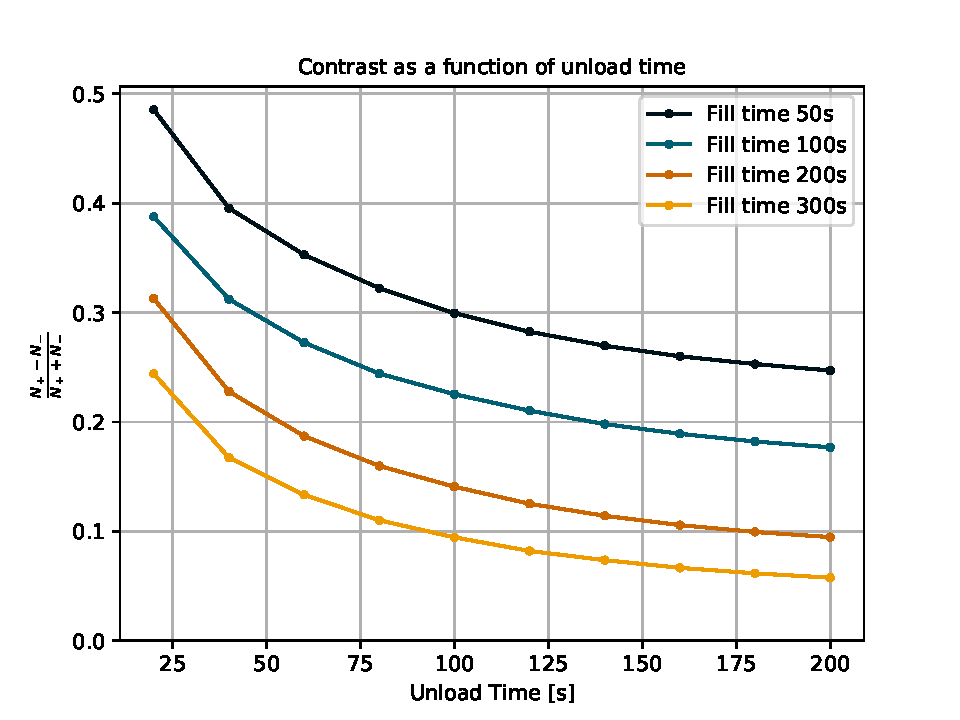
\includegraphics[width=0.6\textwidth]{figures/2021_roundhouse_asymmetry_2.pdf}
    \caption[Depicted is the change in the asymmetry as the roundhouse unload progresses. The $x$-axis refers to the number of integration periods of the run doublet used to calculate asymmetry]
    {Depicted is the change in the asymmetry as the roundhouse unload progresses. The $x$-axis refers to the number of integration periods of the run doublet used to calculate asymmetry (e.g., $\qty{20}{s}=$ first two integration periods,  $\qty{30}{s}=$ first three integration periods...).}\label{fig:2021_roundhouse_asymmetry_2}
\end{figure}